%!TEX root = ../../thesis.tex

%=============================================================================


\section{Interaction between Orchestrator and Library}

Now that we gained deeper insight to both Orchestrator and library, especially with respect to how they solve their respective tasks, we will focus on their interaction and thus give a better impression of the proposed frameworks ''bigger picture''.

% -----------------------------


\begin{figure}[]
	\centering
	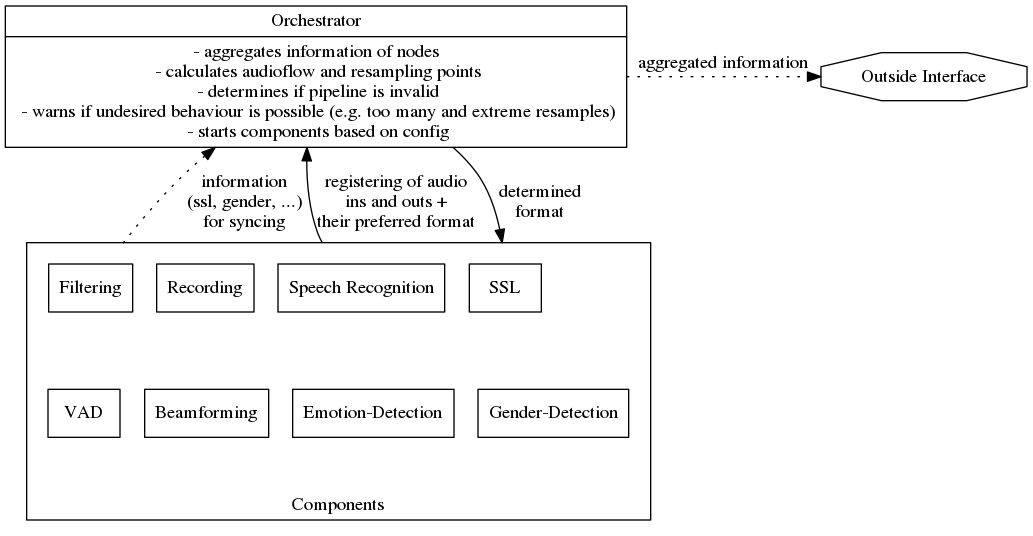
\includegraphics[width=\textwidth]{bilder/graphs/architecture.png}
	\caption{}
	\label{pic:main:combi:arcitecture}
\end{figure}


\begin{itemize}
	\item two main problems: synchronization and transmission/ audio format adjusting
	\item division between library and orchestrator
	\item library as abstraction layer for resampling, transmission and tool to retrieve correlated information, e.g. VAD and SSL results
	\item orchestrator as central control node to manage all participating nodes
	\item ``perspective'' from outside, interfaces into and out of the pipeline
	\item most important ros messages and why they were designed as they were (AugmentedAudio.msg and EsiafRosMsg.msg)
\end{itemize}

general design decisions regarding:

\begin{itemize}
	\item latency
	\item parallelism/ pipeline tree generation
	\item architecture (distributed vs centralized (need for orchestrator))
	\item decision for using ros as an additional middleware (and against jackaudio, gstreamer, alsa, just TCP)
	\item the need for client side selectable audio format 
\end{itemize}

interaction between library and orchestrator

\begin{itemize}
	\item interfaces the orchestrator provides for the clients
\end{itemize}


